\input{header.tex}
\input{newcommands.tex}


\title{Lautschrift mit \hologo{LaTeX} setzen}
\author{Fortbildungsmaterial für Lehrkräfte}
\date{\today}
\pagestyle{plain}
\setlength{\parskip}{1.5em} % Abstand zwischen Absätzen (Handreichungen)
\setlength{\emergencystretch}{2em} % lange \texttt-Wörter umbrechen statt über den Rand


\begin{document}

\maketitle

Vokabellisten mit Aussprache, Material für Deutsch als Zweitsprache, ein Arbeitsblatt zur Phonetik im Deutschunterricht oder die Aussprache englischer Fachbegriffe im Informatikunterricht: Überall braucht man Zeichen des Internationalen Phonetischen Alphabets (IPA). \hologo{LaTeX} bietet dafür zwei Wege, das Paket \texttt{tipa} mit pdflatex oder Unicode-Zeichen mit xelatex. Diese Handreichung erklärt beide, zeigt die wichtigsten Eingaben für Deutsch und Englisch und löst ein Problem, an dem fast alle Anfänger scheitern: Aus der Betonung \ipa{"a} wird plötzlich ein \enquote{ä}.



%%%%  KAPITEL 1  %%%%
\section{Zwei Wege zur Lautschrift}

\begin{center}
\begin{tabular}{@{}l>{\raggedright\arraybackslash}p{6cm}>{\raggedright\arraybackslash}p{6cm}@{}}
	\toprule
	& \textbf{tipa} (pdflatex) & \textbf{Unicode} (xelatex) \\
	\midrule
	Eingabe & Kürzel aus ASCII-Zeichen: \texttt{"mE:tC@n} & Zeichen direkt, wie sie gedruckt werden \\
	Vorteil & läuft in jedem pdflatex-Dokument, auch in bestehenden Arbeitsblättern & gut lesbarer Quelltext; Umschriften aus Wörterbüchern lassen sich kopieren \\
	Nachteil & Kürzel muss man lernen; Konflikt mit \texttt{babel} & braucht eine Schrift mit IPA-Zeichen und einen anderen Compiler \\
	\bottomrule
\end{tabular}
\end{center}

Als Faustregel gilt: Für einzelne Umschriften in einem bestehenden Dokument nimmt man \texttt{tipa}. Für neues Material mit viel Lautschrift, etwa lange Vokabellisten, ist Unicode bequemer. Diese Handreichung ist mit pdflatex gesetzt; alle Ausgaben stammen deshalb aus \texttt{tipa}. Der Unicode-Weg folgt in Kapitel~7.



%%%%  KAPITEL 2  %%%%
\section{Lautschrift mit \texttt{tipa}}


%%%%  UNTERKAPITEL 2.1  %%%%
\subsection{Paket einbinden}

In der universalen \texttt{header.tex} ist \texttt{tipa} bereits geladen. In einem eigenständigen Dokument gehört diese Zeile in die Präambel:

\begin{lstlisting}[style=latex]
\usepackage[safe]{tipa}
\end{lstlisting}

Die Option \texttt{safe} ist wichtig. Ohne sie definiert \texttt{tipa} die Befehle \texttt{\textbackslash;}, \texttt{\textbackslash:}, \texttt{\textbackslash!}, \texttt{\textbackslash*} und \texttt{\textbackslash s} um. Dann bricht zum Beispiel jede Formel mit \texttt{\textbackslash;} als Abstand ab, und den gibt es in fast jeder Mathematik-Lösung.


%%%%  UNTERKAPITEL 2.2  %%%%
\subsection{Die ersten Wörter}

Lautschrift steht im Befehl \texttt{\textbackslash textipa\{\dots\}}. Darin bedeuten Groß- und Sonderzeichen IPA-Zeichen, zum Beispiel \texttt{E} für das offene e \textipa{E}, \texttt{C} für den Ich-Laut \textipa{C} und \texttt{@} für das Schwa \textipa{@}. Ein Doppelpunkt kennzeichnet einen langen Vokal:

\begin{lstlisting}[style=latex]
Lied [\textipa{li:t}], Bett [\textipa{bEt}], ich [\textipa{IC}], Schule [\textipa{Su:l@}], lang [\textipa{laN}]
\end{lstlisting}

\begin{ausgabe}
	Lied [\textipa{li:t}], Bett [\textipa{bEt}], ich [\textipa{IC}], Schule [\textipa{Su:l@}], lang [\textipa{laN}]
\end{ausgabe}



%%%%  KAPITEL 3  %%%%
\section{Betonung und der Konflikt mit \texttt{babel}}

In \texttt{tipa} steht das Anführungszeichen \texttt{"} für den Betonungsstrich \textipa{\textprimstress} vor der betonten Silbe. Mit \texttt{babel} und der Sprache \texttt{ngerman} ist \texttt{"} aber bereits belegt: \texttt{"a} ergibt dort ein \enquote{ä}. Das Ergebnis ist eine falsche Umschrift ohne jede Fehlermeldung:

\begin{lstlisting}[style=latex]
Abend: \textipa{"a:b@nt}  % falsch!
\end{lstlisting}

\begin{ausgabe}
	Abend: \textipa{"a:b@nt}  % falsch!
\end{ausgabe}

Betroffen sind \texttt{"a}, \texttt{"o}, \texttt{"u} und \texttt{"s} (wird zu ß). Bei \texttt{"m} oder \texttt{"k} geht es zufällig gut, deshalb fällt der Fehler oft erst spät auf.

Die Lösung ist der Befehl \texttt{\textbackslash ipa\{\dots\}} aus der universalen \texttt{newcommands.tex}. Er schaltet das Kürzel von \texttt{babel} aus, bevor er die Umschrift liest, und setzt sie gleich in eckige Klammern:

\begin{lstlisting}[style=latex]
Abend: \ipa{"a:b@nt}, Mädchen: \ipa{"mE:tC@n}, Hose: \ipa{"ho:z@}
\end{lstlisting}

\begin{ausgabe}
	Abend: \ipa{"a:b@nt}, Mädchen: \ipa{"mE:tC@n}, Hose: \ipa{"ho:z@}
\end{ausgabe}

In einem eigenständigen Dokument definiert man \texttt{\textbackslash ipa} selbst:

\begin{lstlisting}[style=latex]
\makeatletter
\newcommand\ipa{\begingroup\shorthandoff{"}\ipa@aux}
\newcommand\ipa@aux[1]{[\textipa{#1}]\endgroup}
\makeatother
\end{lstlisting}

\texttt{\textbackslash ipa} wirkt nicht im Argument eines anderen Befehls, etwa in \texttt{\textbackslash textbf\{\dots\}} oder einer Überschrift, weil das Anführungszeichen dort schon gelesen ist. Dort schreibt man den Betonungsstrich als Befehl: \texttt{\textbackslash textprimstress} für die Haupt- und \texttt{\textbackslash textsecstress} für die Nebenbetonung.

\begin{lstlisting}[style=latex]
\textbf{Abend [\textipa{\textprimstress a:b@nt}]}
\end{lstlisting}

\begin{ausgabe}
	\textbf{Abend [\textipa{\textprimstress a:b@nt}]}
\end{ausgabe}



%%%%  KAPITEL 4  %%%%
\section{Die wichtigsten Kürzel}

Die Tabellen zeigen die Laute des Deutschen und des Englischen mit Eingabe und Beispielwort. Eine vollständige Liste steht in der Datei \texttt{tipa-kuerzel.md} im Skill.


%%%%  UNTERKAPITEL 4.1  %%%%
\subsection{Vokale des Deutschen}

\begin{lstlisting}[style=latex]
\begin{tabular}{llll@{\hspace{1cm}}llll}
	\toprule
	Zeichen & Eingabe & Wort & Umschrift & Zeichen & Eingabe & Wort & Umschrift \\
	\midrule
	\textipa{i:}  & \texttt{i:}  & Lied   & \ipa{li:t}   & \textipa{u:} & \texttt{u:} & gut   & \ipa{gu:t} \\
	\textipa{I}   & \texttt{I}   & Mitte  & \ipa{"mIt@}  & \textipa{U}  & \texttt{U}  & Hund  & \ipa{hUnt} \\
	\textipa{y:}  & \texttt{y:}  & müde   & \ipa{"my:d@} & \textipa{o:} & \texttt{o:} & Boot  & \ipa{bo:t} \\
	\textipa{Y}   & \texttt{Y}   & Hütte  & \ipa{"hYt@}  & \textipa{O}  & \texttt{O}  & Sonne & \ipa{"zOn@} \\
	\textipa{e:}  & \texttt{e:}  & Beet   & \ipa{be:t}   & \textipa{\o:} & \texttt{\textbackslash o:} & schön & \ipa{S\o:n} \\
	\textipa{E}   & \texttt{E}   & Bett   & \ipa{bEt}    & \textipa{\oe} & \texttt{\textbackslash oe} & Hölle & \ipa{"h\oe l@} \\
	\textipa{@}   & \texttt{@}   & Hase   & \ipa{"ha:z@} & \textipa{aI} & \texttt{aI} & Eis   & \ipa{aIs} \\
	\textipa{5}   & \texttt{5}   & Lehrer & \ipa{"le:K5} & \textipa{aU} & \texttt{aU} & Haus  & \ipa{haUs} \\
	\textipa{a}   & \texttt{a}   & Mann   & \ipa{man}    & \textipa{OY} & \texttt{OY} & Leute & \ipa{"lOYt@} \\
	\bottomrule
\end{tabular}
\end{lstlisting}

\begin{ausgabe}
	\centering
	\begin{tabular}{llll@{\hspace{1cm}}llll}
		\toprule
		Zeichen & Eingabe & Wort & Umschrift & Zeichen & Eingabe & Wort & Umschrift \\
		\midrule
		\textipa{i:}  & \texttt{i:}  & Lied   & \ipa{li:t}   & \textipa{u:} & \texttt{u:} & gut   & \ipa{gu:t} \\
		\textipa{I}   & \texttt{I}   & Mitte  & \ipa{"mIt@}  & \textipa{U}  & \texttt{U}  & Hund  & \ipa{hUnt} \\
		\textipa{y:}  & \texttt{y:}  & müde   & \ipa{"my:d@} & \textipa{o:} & \texttt{o:} & Boot  & \ipa{bo:t} \\
		\textipa{Y}   & \texttt{Y}   & Hütte  & \ipa{"hYt@}  & \textipa{O}  & \texttt{O}  & Sonne & \ipa{"zOn@} \\
		\textipa{e:}  & \texttt{e:}  & Beet   & \ipa{be:t}   & \textipa{\o:} & \texttt{\textbackslash o:} & schön & \ipa{S\o:n} \\
		\textipa{E}   & \texttt{E}   & Bett   & \ipa{bEt}    & \textipa{\oe} & \texttt{\textbackslash oe} & Hölle & \ipa{"h\oe l@} \\
		\textipa{@}   & \texttt{@}   & Hase   & \ipa{"ha:z@} & \textipa{aI} & \texttt{aI} & Eis   & \ipa{aIs} \\
		\textipa{5}   & \texttt{5}   & Lehrer & \ipa{"le:K5} & \textipa{aU} & \texttt{aU} & Haus  & \ipa{haUs} \\
		\textipa{a}   & \texttt{a}   & Mann   & \ipa{man}    & \textipa{OY} & \texttt{OY} & Leute & \ipa{"lOYt@} \\
		\bottomrule
	\end{tabular}
\end{ausgabe}

Nach Befehlen wie \texttt{\textbackslash oe} oder \texttt{\textbackslash o} steht ein Leerzeichen, wenn ein Buchstabe folgt: \texttt{h\textbackslash oe l@}. Sonst liest \hologo{LaTeX} \texttt{\textbackslash oel} als einen unbekannten Befehl.


%%%%  UNTERKAPITEL 4.2  %%%%
\subsection{Konsonanten des Deutschen}

\begin{lstlisting}[style=latex]
\begin{tabular}{llll@{\hspace{1cm}}llll}
	\toprule
	Zeichen & Eingabe & Wort & Umschrift & Zeichen & Eingabe & Wort & Umschrift \\
	\midrule
	\textipa{C} & \texttt{C} & ich    & \ipa{IC}       & \textipa{K}  & \texttt{K}  & Rose    & \ipa{"Ko:z@} \\
	\textipa{x} & \texttt{x} & Bach   & \ipa{bax}      & \textipa{P}  & \texttt{P}  & beachten & \ipa{b@"Paxt\textsyllabic{n}} \\
	\textipa{S} & \texttt{S} & Schule & \ipa{"Su:l@}   & \textipa{ts} & \texttt{ts} & Zeit    & \ipa{tsaIt} \\
	\textipa{Z} & \texttt{Z} & Garage & \ipa{ga"Ka:Z@} & \textipa{pf} & \texttt{pf} & Apfel   & \ipa{"apf\textsyllabic{l}} \\
	\textipa{N} & \texttt{N} & lang   & \ipa{laN}      & \textipa{tS} & \texttt{tS} & deutsch & \ipa{dOYtS} \\
	\bottomrule
\end{tabular}
\end{lstlisting}

\begin{ausgabe}
	\centering
	\begin{tabular}{llll@{\hspace{1cm}}llll}
		\toprule
		Zeichen & Eingabe & Wort & Umschrift & Zeichen & Eingabe & Wort & Umschrift \\
		\midrule
		\textipa{C} & \texttt{C} & ich    & \ipa{IC}       & \textipa{K}  & \texttt{K}  & Rose    & \ipa{"Ko:z@} \\
		\textipa{x} & \texttt{x} & Bach   & \ipa{bax}      & \textipa{P}  & \texttt{P}  & beachten & \ipa{b@"Paxt\textsyllabic{n}} \\
		\textipa{S} & \texttt{S} & Schule & \ipa{"Su:l@}   & \textipa{ts} & \texttt{ts} & Zeit    & \ipa{tsaIt} \\
		\textipa{Z} & \texttt{Z} & Garage & \ipa{ga"Ka:Z@} & \textipa{pf} & \texttt{pf} & Apfel   & \ipa{"apf\textsyllabic{l}} \\
		\textipa{N} & \texttt{N} & lang   & \ipa{laN}      & \textipa{tS} & \texttt{tS} & deutsch & \ipa{dOYtS} \\
		\bottomrule
	\end{tabular}
\end{ausgabe}

\texttt{K} ist das Zäpfchen-R \textipa{K}, wie es im Deutschen meist gesprochen wird, \texttt{P} der Knacklaut vor Vokalen am Wort- oder Silbenanfang.


%%%%  UNTERKAPITEL 4.3  %%%%
\subsection{Eine Vokabelliste für Englisch}

Für Englisch kommen einige Zeichen hinzu, etwa \texttt{T} und \texttt{D} für die beiden th-Laute, \texttt{\textbackslash ae} für den Laut in \textit{cat} und \texttt{\textbackslash textturnr} für das englische r. Eine Vokabelliste mit Aussprache:

\begin{lstlisting}[style=latex]
\begin{tabular}{lll}
	\toprule
	\textbf{Englisch} & \textbf{Aussprache} & \textbf{Deutsch} \\
	\midrule
	thought  & \ipa{TO:t}         & Gedanke \\
	the      & \ipa{D@}           & der, die, das \\
	cat      & \ipa{k\ae t}       & Katze \\
	cup      & \ipa{k2p}          & Tasse \\
	bird     & \ipa{b3:d}         & Vogel \\
	red      & \ipa{\textturnr ed} & rot \\
	measure  & \ipa{"meZ@}        & messen \\
	computer & \ipa{k@m"pju:t@}   & Rechner \\
	\bottomrule
\end{tabular}
\end{lstlisting}

\begin{ausgabe}
	\centering
	\begin{tabular}{lll}
		\toprule
		\textbf{Englisch} & \textbf{Aussprache} & \textbf{Deutsch} \\
		\midrule
		thought  & \ipa{TO:t}         & Gedanke \\
		the      & \ipa{D@}           & der, die, das \\
		cat      & \ipa{k\ae t}       & Katze \\
		cup      & \ipa{k2p}          & Tasse \\
		bird     & \ipa{b3:d}         & Vogel \\
		red      & \ipa{\textturnr ed} & rot \\
		measure  & \ipa{"meZ@}        & messen \\
		computer & \ipa{k@m"pju:t@}   & Rechner \\
		\bottomrule
	\end{tabular}
\end{ausgabe}



%%%%  KAPITEL 5  %%%%
\section{Zusatzzeichen und Langformen}

Außer den Buchstaben gibt es Zeichen für Länge, Betonung und besondere Aussprache. Weil die Option \texttt{safe} die Kurzformen \texttt{\textbackslash s}, \texttt{\textbackslash *} und \texttt{\textbackslash ;} abschaltet, verwendet man immer die Langformen:

\begin{lstlisting}[style=latex]
\begin{tabular}{lll}
	\toprule
	\textbf{Zeichen} & \textbf{Eingabe} & \textbf{Bedeutung} \\
	\midrule
	\ipa{"ha:b\textsyllabic{n}}    & \verb|\textsyllabic{n}| & silbisches n (haben) \\
	\ipa{a:} \ipa{a}               & \verb|:|                & lang und kurz \\
	\ipa{"a:b\textsyllabic{n}t""PEs\textsyllabic{n}} & \verb|"| und \verb|""| & Haupt- und Nebenbetonung (Abendessen) \\
	\ipa{bl\~a}                    & \verb|\~a|              & nasal (franz.\ blanc) \\
	\ipa{\textturnr}               & \verb|\textturnr|       & englisches r \\
	\ipa{\textscr}                 & \verb|\textscr|         & gerolltes Zäpfchen-R \\
	\ipa{\textsubring{n}}          & \verb|\textsubring{n}|  & stimmlos (nicht silbisch!) \\
	\bottomrule
\end{tabular}
\end{lstlisting}

\begin{ausgabe}
	\centering
	\begin{tabular}{lll}
		\toprule
		\textbf{Zeichen} & \textbf{Eingabe} & \textbf{Bedeutung} \\
		\midrule
		\ipa{"ha:b\textsyllabic{n}}    & \verb|\textsyllabic{n}| & silbisches n (haben) \\
		\ipa{a:} \ipa{a}               & \verb|:|                & lang und kurz \\
		\ipa{"a:b\textsyllabic{n}t""PEs\textsyllabic{n}} & \verb|"| und \verb|""| & Haupt- und Nebenbetonung (Abendessen) \\
		\ipa{bl\~a}                    & \verb|\~a|              & nasal (franz.\ blanc) \\
		\ipa{\textturnr}               & \verb|\textturnr|       & englisches r \\
		\ipa{\textscr}                 & \verb|\textscr|         & gerolltes Zäpfchen-R \\
		\ipa{\textsubring{n}}          & \verb|\textsubring{n}|  & stimmlos (nicht silbisch!) \\
		\bottomrule
	\end{tabular}
\end{ausgabe}

Vorsicht: Im \texttt{safe}-Modus ergeben die Kurzformen \texttt{\textbackslash *r} und \texttt{\textbackslash ;R} \textit{ohne} Fehlermeldung ein falsches Zeichen, nämlich ein gewöhnliches r. Deshalb nur die Langformen aus der Tabelle verwenden.



%%%%  KAPITEL 6  %%%%
\section{Das Vokalviereck}

Das Vokalviereck ordnet die Vokale nach der Lage der Zunge: links vorn, rechts hinten, oben geschlossen, unten offen. Links von einem Punkt steht der ungerundete, rechts der gerundete Vokal. Mit \TikZ und \texttt{\textbackslash textipa} lässt es sich direkt zeichnen. Die Linien beginnen erst hinter den Zeichen rechts der Punkte, damit sie diese nicht durchstreichen:

\begin{lstlisting}[style=latex]
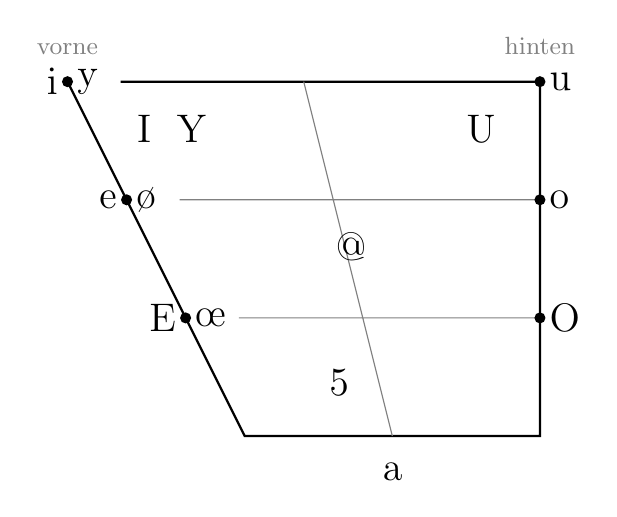
\begin{tikzpicture}[x=1.5cm, y=1.5cm, every node/.style={font=\Large}]
	% Trapez; die Linien beginnen erst hinter den Zeichen rechts der Punkte
	\draw[thick] (0.45,3) -- (4,3) -- (4,0) -- (1.5,0) -- (0,3);
	\draw[gray] (0.95,2) -- (4,2)  (1.45,1) -- (4,1)  (2,3) -- (2.75,0);
	% links vom Punkt ungerundet, rechts gerundet
	\foreach \x/\y/\u/\g in {0/3/i/y, 0.5/2/e/\o, 1/1/E/\oe, 4/3//u, 4/2//o, 4/1//O}{
		\fill (\x,\y) circle (2pt);
		\node[left]  at (\x,\y) {\textipa{\u}};
		\node[right] at (\x,\y) {\textipa{\g}};}
	\node at (0.65,2.6) {\textipa{I}};  \node at (1.05,2.6) {\textipa{Y}};
	\node at (3.5,2.6)  {\textipa{U}};  \node at (2.4,1.6)  {\textipa{@}};
	\node at (2.3,0.45) {\textipa{5}};  \node at (2.75,-0.3) {\textipa{a}};
	\node[font=\small, gray, above] at (0,3.15) {vorne};
	\node[font=\small, gray, above] at (4,3.15) {hinten};
\end{tikzpicture}
\end{lstlisting}

\begin{ausgabe}
	\centering
	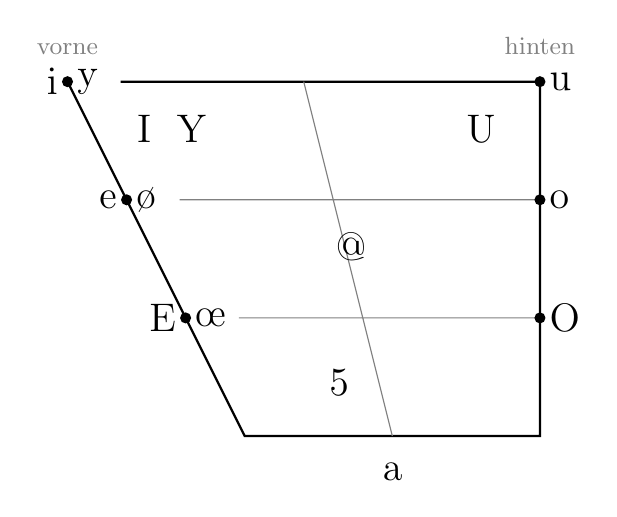
\begin{tikzpicture}[x=1.5cm, y=1.5cm, every node/.style={font=\Large}]
		% Trapez; die Linien beginnen erst hinter den Zeichen rechts der Punkte
		\draw[thick] (0.45,3) -- (4,3) -- (4,0) -- (1.5,0) -- (0,3);
		\draw[gray] (0.95,2) -- (4,2)  (1.45,1) -- (4,1)  (2,3) -- (2.75,0);
		% links vom Punkt ungerundet, rechts gerundet
		\foreach \x/\y/\u/\g in {0/3/i/y, 0.5/2/e/\o, 1/1/E/\oe, 4/3//u, 4/2//o, 4/1//O}{
			\fill (\x,\y) circle (2pt);
			\node[left]  at (\x,\y) {\textipa{\u}};
			\node[right] at (\x,\y) {\textipa{\g}};}
		\node at (0.65,2.6) {\textipa{I}};  \node at (1.05,2.6) {\textipa{Y}};
		\node at (3.5,2.6)  {\textipa{U}};  \node at (2.4,1.6)  {\textipa{@}};
		\node at (2.3,0.45) {\textipa{5}};  \node at (2.75,-0.3) {\textipa{a}};
		\node[font=\small, gray, above] at (0,3.15) {vorne};
		\node[font=\small, gray, above] at (4,3.15) {hinten};
	\end{tikzpicture}
\end{ausgabe}



%%%%  KAPITEL 7  %%%%
\section{Der Unicode-Weg mit xelatex}

Mit xelatex (oder lualatex) schreibt man die Lautzeichen direkt in den Quelltext, zum Beispiel kopiert von \texttt{ipa.typeit.org}. Dafür braucht man eine Schrift, die alle IPA-Zeichen enthält. Gut geeignet und kostenlos sind \textit{Charis SIL}, \textit{Doulos SIL} und \textit{Gentium Plus} (\texttt{software.sil.org}). Das Grundgerüst:

\begin{lstlisting}[style=latex, escapechar=!]
\documentclass[11pt,a4paper]{article}
\usepackage{fontspec}
\usepackage[ngerman]{babel}
\setmainfont{Charis SIL}
\newcommand\ipa[1]{[#1]}

\begin{document}
Mädchen \ipa{!\textipa{\textprimstress mE:tC@n}!}, Abend \ipa{!\textipa{\textprimstress a:b\textsyllabic{n}t}!}, thing \ipa{!\textipa{TIN}!}
\end{document}
\end{lstlisting}

Ein Konflikt mit \texttt{babel} entsteht hier nicht, weil der Betonungsstrich ein eigenes Zeichen ist. Das Dokument muss aber mit \texttt{xelatex} statt \texttt{pdflatex} übersetzt werden. Fehlt der Schrift ein Zeichen, bleibt im PDF eine Lücke; im Protokoll (\texttt{.log}) steht dann \enquote{Missing character}. Ein vollständiges Beispiel mit Vokalviereck liegt im Skill als \texttt{vorlage\_lautschrift\_unicode.tex}.



%%%%  KAPITEL 8  %%%%
\section{Zusammenfassung}

Die wichtigsten Techniken im Überblick:

\begin{itemize}
	\item \texttt{tipa} immer mit der Option \texttt{safe} laden, sonst funktionieren \texttt{\textbackslash;} und andere Befehle nicht mehr.
	\item Umschriften mit Betonung nicht mit \texttt{\textbackslash textipa}, sondern mit \texttt{\textbackslash ipa\{\dots\}} setzen, sonst wird \texttt{"a} zu \enquote{ä}.
	\item In Überschriften und Befehlsargumenten den Betonungsstrich als \texttt{\textbackslash textprimstress} schreiben.
	\item Langformen wie \texttt{\textbackslash textsyllabic\{n\}} und \texttt{\textbackslash textturnr} statt der Kurzformen verwenden.
	\item Für viel Lautschrift den Unicode-Weg mit xelatex und einer SIL-Schrift wählen.
\end{itemize}

Lautschrift sieht man Fehler im Quelltext kaum an. Deshalb sollte man jede Umschrift im fertigen PDF mit dem Beispielwort vergleichen, bevor das Material in die Klasse geht.

\end{document}
